\documentclass[11pt]{article}
\usepackage[letterpaper, margin=1in]{geometry}

% Proper links
\usepackage[
    pdftitle={SYSC3010 Computer Systems Development Project - FANS Project Proposal},
    colorlinks=false,
    allbordercolors={0 0 0},
    citebordercolor={1 1 1}, % No border for citations
    pdfborderstyle={/S/U/W 1},
]{hyperref}

% Display graphics nicely
\usepackage{float}
\usepackage{graphicx}

% References
\usepackage[style=ieee]{biblatex}
\addbibresource{./references.bib}

% Remove paragraph indentation and use newline to separate instead. %
\usepackage[parfill]{parskip}
\setlength{\parindent}{0cm}

\author{
    Grant Achuzia, 101222695 \\
    Javeria Sohail, 101197163 \\
    Matteo Golin, 101220709 \\
    Saja Fawagreh, 101217326 \\
    TA: Sean Kirkby
}
\title{
    SYSC3010 Computer Systems Development Project \\
    FANS Project Proposal \\
    {\large Group L1-G8} \\
    {
        \vspace{0.5in}
        \centering
        
\includegraphics[width=4in]{../assets/header-image.jpg} \\
        \small \cite{header-img}
    }
}
\date{
    Created: February 11th, 2024 \\
    Modified: \today
}

\begin{document}

% TITLE %
\maketitle
\pagebreak

% TABLE OF CONTENTS %
{
    \hypersetup{hidelinks}
    \tableofcontents
}

% MAIN MATTER %
\section{Project Description}

\subsection{Motivation}

The motivation for the FANS project was to address the critical problem of preventable fire-related deaths in Canada.
Fire safety was a fundamental concern for individuals, families, and communities nationwide. By leveraging modern
technological advancements, the FANS system aimed to significantly enhance the effectiveness of fire alarm systems,
reducing response times, and ultimately saving lives. The importance of this project could not be overstated, as it
directly impacted the safety and well-being of Canadians.

\subsection{Problem Statement}

The need for the Fire Alarm Notification System (FANS) stemmed from the alarming number of preventable fire deaths in
Canada, where 220 people died in fires each year, with at least one in seven of these deaths occurring in homes without
working smoke alarms \cite{fire-stats}. This critical problem underscored the shortcomings of traditional fire alarm
systems, which often lacked advanced communication capabilities and real-time monitoring capabilities
\cite{modern-fire-alarms}. These limitations not only contributed to delayed response times but also to preventable
deaths, underscoring the urgent need for an advanced fire alarm solution.

Traditional systems’ shortcomings, coupled with the fact that smoke detection systems were sometimes unsafely disarmed
by users to avoid false alarms—especially those installed close to kitchen spaces—further exacerbated the problem. The
FANS project sought to address these issues by integrating smoke and temperature sensors with Internet of Things (IoT)
technology. This approach not only aimed to cover scenarios where smoke may not reach the detecting device but also
offered real-time notifications via SMS and email, thus notifying homeowners immediately in the event of an emergency.

By providing configurable thresholds for smoke and temperature alarms and adjustable timeouts that prevented the system
from being deactivated in an unsafe manner, FANS aimed to use technological advances to significantly improve the
effectiveness of fire detection systems. The ultimate goal of the project was to reduce response times, improve overall
fire safety, and thereby mitigate fire disasters and protect the well-being of individuals, families, and communities
across Canada \cite{smoke-alarm-gc}.

\subsection{Overview of Solution}

\section{System Design}

\subsection{System Overview Diagram}

Figure \ref{fig:deployment} shows the deployment diagram for FANS. There will be three devices which communicate with
each other on a local network:

\begin{enumerate}
    \item The alarm system on a Raspberry Pi 4.
    \item The smoke detection system on a Raspberry Pi 4.
    \item A notification system on a Raspberry Pi 4.
\end{enumerate}

\begin{figure}[H]
    \centering
    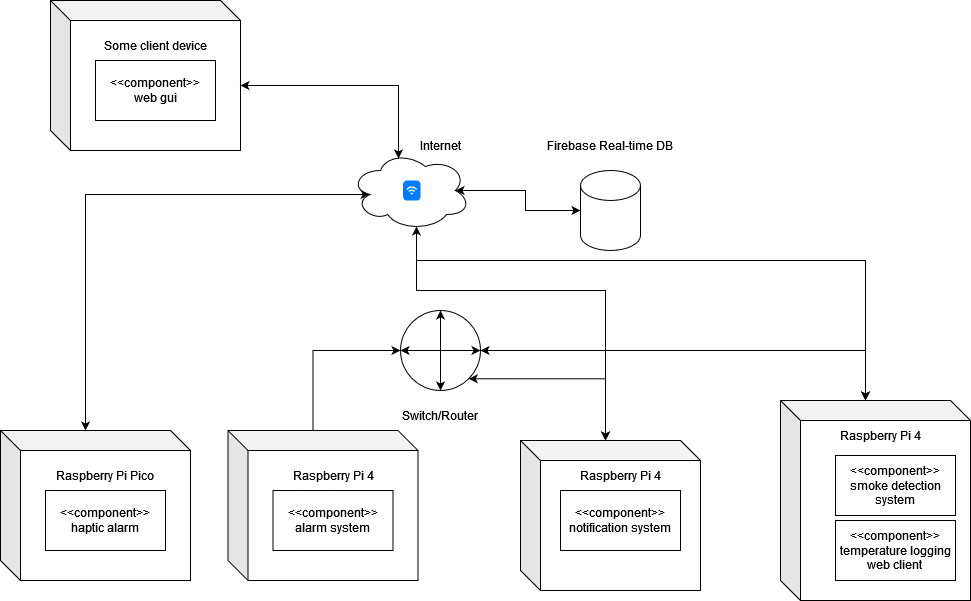
\includegraphics[width=\linewidth]{../assets/FANSDeployment.png}
    \caption{Deployment diagram of FANS.}
    \label{fig:deployment}
\end{figure}

The smoke detection and temperature logging system will continuously update the cloud database with recorded smoke and
temperature levels.

When the smoke detection system detects a smoke or temperature measurement above the limiting threshold, it will signal
the alarm system to sound the alarm using a UDP packet. It will also signal the notification system to send out
notifications to the subscriber list in the same way, and then send a write request to the cloud database to signal the
emergency detection flag.

The fourth device, the Pi Pico, will buzz when the cloud database indicates that an emergency has been detected by the
detection system. This will physically notify the user of the emergency.

The notification and alarm system are on separate devices to preserve their integrity in the case of an emergency. It
is possible that the smoke detection system will be closer to the source of the fire, and therefore be at risk of being
damaged/disabled. With the notification and alarm systems on separate devices connected through a local internet
connection, they will be able to perform their responsibilities with less risk of being damaged by flames. The local
connection also allows the alarm to sound in the case where the local network loses internet connection.

The cloud database is a real-time database to facilitate the real-time nature of display information on the web GUI. In
addition, it will allow the haptic feedback device to buzz as soon as the smoke detection system signals an emergency
to the cloud database. The fire alarm system has a real-time nature which needs to be preserved.

The web GUI will be served on the cloud, allowing us to serve our interface to multiple users more easily.

\textbf{Scalability} \\
This configuration would allow us to scale our system horizontally very easily. Multiple different alarm systems and
smoke detectors could be connected over a local network to a notification system, allowing smoke detection in multiple
rooms and alarms sounding in multiple rooms. Additionally, several haptic alarm wearable devices could be clients to
the real-time database, allowing any number of users to be notified haptically in the event of an emergency.

\textbf{Modularity} \\
Each subsystem has a single responsibility that allows for modularity in FANS. Subsystems have a clearly defined
interface with specific messages passed between them, allowing subsystems to operate without knowledge of each others’
implementations.

The smoke detection system simply sends emergency signals out over the local network to nodes who are listening, which
allows it to set off multiple alarm nodes.

The cloud database makes data available in such a way that multiple web UI clients and multiple wearable devices can
access sensor data and emergency flags.

The notification system is entirely self-contained, and only requires access to contact information in the cloud
database.

\subsubsection{Communication Protocols}

The smoke detection system will be communicating with an array of temperature and smoke sensors using the I2C protocol
over the GPIO pins of a Raspberry Pi 4.

Each node on the local network (the smoke detection system, alarm system and notification system) will communicate with
each other using UDP packets over the local network.

Nodes which communicate with the cloud hosted real-time Firebase database will use HTTP requests to interact with the
database.

\begin{itemize}
    \item The smoke detection system will post JSON payloads to the database to write data.
    \item The web GUI will request JSON over HTTP to update its visual components (dashboard with charts, etc.) with the data
          stored in the database.
    \item The notification system will request contact information from the database over HTTP to send notifications to affected
          users.
    \item The haptic alarm system will poll a database flag over HTTP to check if there is an active emergency.
\end{itemize}

Finally, the notification system will communicate with affected users over email and SMS text notifications. This will
use standard internet, SMS and email protocols.

\subsection{Component Details}

The following section will describe the interfaces and responsibilities of each major node in the FANS system.

\subsubsection{Smoke Detection System}

The first component in the proposed system is the smoke detection and temperature sensing system. It will read sensor
data from a locally connected smoke sensor and temperature sensor using the I2C protocol over the Raspberry Pi 4's GPIO
pins. It will then update the real-time Firebase database with the collected sensor data over an internet connection.

If any temperature or smoke measurements are above the critical threshold for signalling an emergency, it will send a
message to the notification system and the alarm system over UDP to signify an emergency. It will also update a flag in
the real-time database to signify that an emergency has been detected.

The smoke detection system can be configured by the user. The user configuration settings will be read from the cloud
database whenever they are updated, which allows the smoke detection system to use configurable smoke and temperature
thresholds and have a time-out.

\begin{figure}[H]
    \centering
    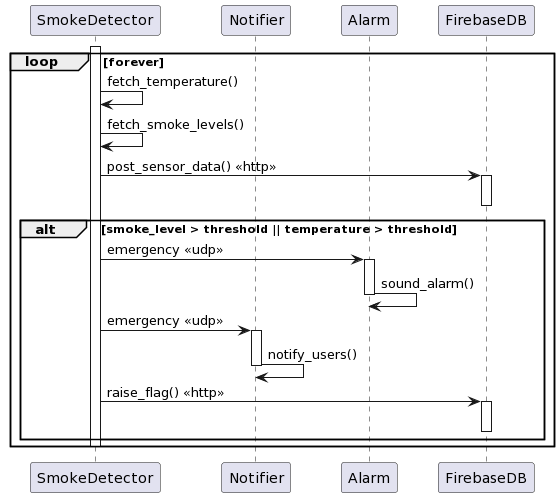
\includegraphics[width=5in]{../assets/SmokeDetectorSequence.png}
    \caption{Sequence diagram for the primary responsibilities of the smoke detector system.}
    \label{fig:smoke-detector-sq}
\end{figure}

\subsubsection{Notification System}

The notification system is responsible for notifying affected users of an emergency and triggering the alarm system. It
will also send SMS and email notifications to all users in the database to notify them of the detected emergency.

The notification system sends its notifications following the receipt of a UDP message from the smoke detection system.
The contact information of the notification recipients are stored both on its local database and the cloud database.
The local database is synchronized periodically with the cloud.

\subsubsection{Alarm System}

The alarm system is responsible for sounding an alarm in the building when an emergency has been detected. The alarm
system receives notification over UDP from the smoke detection system when an emergency has been detected, at which
point it sounds an alarm and flashes lights.

The lights will be an on-board SenseHat, and the alarm is an audio-hat module. The alarm will continue to sound until
the system receives a UDP message to stop.

\subsubsection{Haptic Alarm System}

The haptic alarm system is designed to be a wearable device that vibrates during an emergency. The device queries the
real-time database for a flag indicating an alarm. Once the flag is raised, the device vibrates until the emergency has
ended (the flag is "lowered" in the database).

\begin{figure}[H]
    \centering
    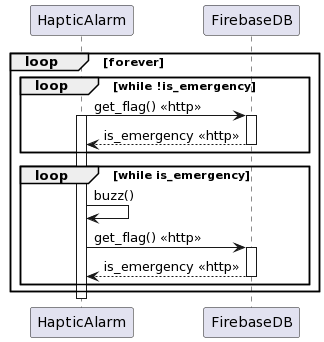
\includegraphics[width=3in]{../assets/HapticAlarmSequence.png}
    \caption{Sequence diagram for the primary responsibilities of the haptic alarm system.}
    \label{fig:haptic-alarm-sq}
\end{figure}

\subsubsection{Firebase Real-Time Database}

The real-time database is responsible for storing smoke and temperature level data in real-time, as well as a database
flag indicating emergency. User contact information will also be stored in this database. Finally, it will also contain
user-configured settings (such as smoke level threshold for triggering an emergency). It will be cloud hosted by
Firebase.

The interaction between the haptic alarm system and the real-time database is visible in Figure
\ref{fig:haptic-alarm-sq}. The interaction between the smoke detector system and the real-time database is visible in
Figure \ref{fig:smoke-detector-sq}. The primary interaction between the web GUI and the real-time database is
documented in Figure \ref{fig:webui-sq}, and secondary interactions can be seen in Section \ref{s:use-cases}.

\subsubsection{Web GUI}

The web GUI is responsible for displaying the sensor information from the real-time database on time-series charts. It
will also allow users to configure settings for FANS (emergency thresholds, etc.) and add more user contact information
to the notification subscriber list. It will also allow users to disable the alarm when an emergency has been resolved.

\begin{figure}[H]
    \centering
    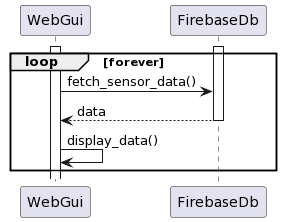
\includegraphics[width=3in]{../assets/WebGUiSequence.png}
    \caption{Sequence diagram for the primary responsibilities of web GUI.}
    \label{fig:webui-sq}
\end{figure}

\subsection{Use Cases} \label{s:use-cases}

\subsubsection{Adding New Contact Information}

\textbf{Actor:} User

\textbf{Preconditions:}
\begin{itemize}
    \item User must be logged into the Web GUI.
    \item user must be authenticated and authorized to make database changes.
\end{itemize}

\textbf{Flow of events:}
\begin{enumerate}
    \item User accesses the web GUI.
    \item User navigates to the section for managing contacts or settings.
    \item User selects the option to add new contact information.
    \item User fills in the required fields such as name, phone number, and email address.
    \item User submits the form to save the new contact information.
    \item The web GUI sends a request to the Firebase Real-Time Database to add the new contact information.
    \item Firebase Real-Time Database confirms the successful addition of the new contact information.
    \item The web GUI displays a confirmation message to the user indicating that the new contact information has been
          successfully added.
\end{enumerate}

\textbf{Postconditions:}
\begin{itemize}
    \item The new contact information is stored in the Firebase Real-Time Database.
    \item The web GUI reflects the updated contact list.
\end{itemize}

\begin{figure}[H]
    \centering
    \includegraphics[width=\linewidth]{../assets/AddContactInfo.png}
    \caption{Sequence diagram for the major interactions in the "Add Contact Information" use case.}
\end{figure}

\subsubsection{Change Emergency Threshold}

\textbf{Actor:} User

\textbf{Preconditions:}
\begin{itemize}
    \item User must have access to the web GUI.
    \item User must be authenticated and authorized to make changes to the database.
    \item The smoke detection system must be operational and connected to the Firebase Real-Time Database.
\end{itemize}

\textbf{Flow of events:}
\begin{enumerate}
    \item User accesses the web GUI.
    \item User navigates to the section for managing settings.
    \item User selects the option to change the smoke detection threshold.
    \item User enters the new threshold value.
    \item User submits the form to save the new threshold value.
    \item The web GUI sends a request to the Firebase Real-Time Database to update the smoke detection threshold.
    \item Firebase Real-Time Database confirms the successful update of the threshold value.
    \item The web GUI displays a confirmation message to the user indicating that the threshold value has been successfully
          updated.
\end{enumerate}

\textbf{Postconditions:}
\begin{itemize}
    \item The new smoke detection threshold value is stored in the Firebase Real-Time Database.
    \item The smoke detection system adjusts its threshold for triggering an emergency based on the new value.
    \item The web GUI reflects the updated threshold value.
\end{itemize}

% TODO: The sequence diagrams are missing activations
\begin{figure}[H]
    \centering
    \includegraphics[width=\linewidth]{../assets/ChangeThresholdUseCaseSequence.png}
    \caption{Sequence diagram for the major interactions in the "Change Emergency Threshold" use case.}
\end{figure}

\subsubsection{Trigger Emergency}

\textbf{Flow of events}
\begin{enumerate}
    \item The smoke detection system sends a TCP message to the notification system to warn of an emergency.
    \item The smoke detection system raises a flag in the real-time database to indicate the emergency.
    \item The notification system forwards this message to the alarm system.
    \item The notification system begins sending SMS and email notifications to the users who are listed in the database.
    \item The alarm system receives the TCP message from the notification system.
    \item The alarm system sounds the alarm and flashes LEDs.
    \item The haptic alarm system reads the flag from the real-time database.
    \item The haptic alarm system begins buzzing.
\end{enumerate}

\begin{figure}[H]
    \centering
    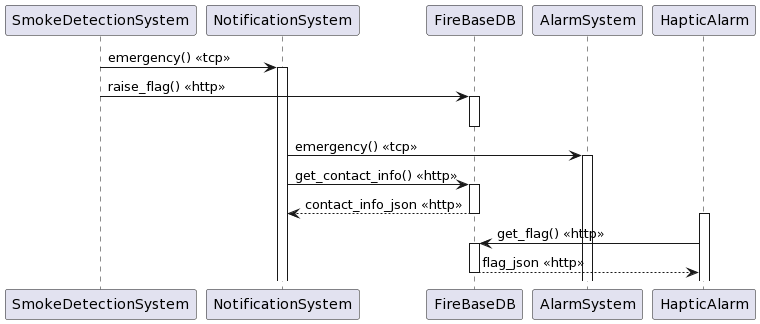
\includegraphics[width=\linewidth]{../assets/FANSAlarmUseCaseSequence.png}
    \caption{Sequence diagram for the major interactions in the "Trigger Emergency" use case.}
\end{figure}

\section{Work Plan}

The following section describes the approach taken by the FANS development team to collaborate effectively and complete
the FANS system before its deadline.

\subsection{The Project Team}

Each member of the project team is a third year computer systems engineering student.

\textbf{Grant Achuzia} \\
Grant's strengths lie in effective project management and organization, and he is passionate about delivering successful
projects in academic settings. Grant also has significant experience designing web interfaces that are accessible and
aesthetically pleasing.

\textbf{Matteo Golin} \\
Matteo has background in developing embedded system on Raspberry Pi's from his work at Carleton University's rocketry
design team, where he is leading the development of a real-time telemetry system using Blackberry's QNX RTOS.

\textbf{Saja Fawagreh} \\
Saja has developed skills in user interface design from her time on co-op, and excels and making visually appealing
interfaces because of her sharp attention to detail.

\textbf{Javeria Sohail} \\
Javeria has expertise in system architecture design, and has a strong knowledge of object-oriented design patterns. She
is passionate about optimization, efficient design and modularity.

\subsubsection{Roles and Tasks}

% TODO: modify responsibilities
\begin{table}[H]
    \centering
    \begin{tabular}{| c | p{3cm} | p{4cm} | p{5cm} |}
        \hline
        \textbf{Team Member} & \textbf{Major Role/Task (Primary)} & \textbf{Secondary Responsibility (Testing)} &
        \textbf{Reason for assignment}                                                                                                  \\
        \hline
        Grant Achuzia        & User interface design              & Local network communication                 & Very
        familiar with HTML/CSS/JavaScript and has knowledge of good web design practices.                                               \\
        \hline
        Matteo Golin         & Sensor data collection             & Local network communication                 &
        Experience writing software to drive sensors and collect data from them because of his experience with CU
        InSpace. Familiar with networking protocols from 5G automation co-op at DELL Technologies.                                      \\
        \hline
        Saja Fawagreh        & Notification system                & Local network communication                 &
        Good communicator, capable of writing succinct Python logic for accomplishing the task.                                         \\
        \hline
        Javeria Sohail       & Haptic alarm system                & Local network communication                 & Familiar with LED and
        buzzer actuators from SYSC3310.                                                                                                 \\
        \hline
    \end{tabular}
    \caption{Assignment of team members to major project tasks}
\end{table}

\subsubsection{Teamwork Strategy}

\textbf{Regular Team Meetings} \\
We will schedule regular team meetings to discuss project progress, share updates, and address any challenges or
questions. Our team will establish MS Teams as our main communication channel to ensure efficient communication within
the team and with the TA.

Additionally, the team meetings will be documented to review what we talked about in the case that someone misses a
meeting.

\textbf{Version Control} \\
We will use GitHub to manage our codebase changes. This will include practices such as creating branches for features or bug
fixes, committing regularly, and requiring code reviews before merging pull requests.

Informative commit messages that follow the SYSC3010 commit formatting guidelines will be required to avoid
misunderstandings.

The team will release frequent prototypes using GitHub's version release features. Versioning will follow
\textit{semantic versioning} (semver) notation. \cite{semver}

\textbf{Code Reviews} \\
Before merging code changes, thorough code reviews will be conducted to ensure code quality and maintainability, as well
as gain feedback about feature implementations from other team members.

\textbf{Testing} \\
We will follow a testing strategy that includes unit testing, integration testing, and system testing to ensure the
reliability and robustness of the FANS.

FANS will be frequently prototyped to ensure a working system at each development step. This methodology is in
accordance with the V-model. \cite{v-model} To ensure this, mocking will be used to simulate modules of the system that
haven't been fully implemented.

Unit testing will be written by developers who have written the feature under test, and will also be run as GitHub
workflows on pull requests to ensure that new code does not break existing functionality.

\textbf{Feedback} \\
Team members will provide constructive feedback to each other for continuous improvement and learning (also making use
of Feedback Fruits). We will also request feedback from our TA at every milestone so that our final system comes together
seamlessly.

\subsubsection{What We Will Need to Learn}

\textbf{Hardware integration} \\
Since the FANS includes both hardware and software components, we need to learn how to integrate them seamlessly. We
utilize online resources and forums where hardware integration techniques are discussed. Many of our hardware modules
(SenseHat, AudioHat, etc.) have associated online tutorials and a plethora of information associated with them.
\cite{sensehat} We will leverage this information.

\textbf{Real-time communication} \\
Implementing real-time communication features such as SMS and email notifications requires
knowledge of APIs and protocols for sending messages. We will look at the documentation and instructions provided by
communication service providers (e.g. SMS) and learn how to integrate these services into our system.

We will also seek out Python tutorials for automated email sending, as there are several Python libraries that provide
this functionality (such as \texttt{smtplib} \cite{python-email}).

\textbf{Developing a web interface} \\
Creating a user-friendly web interface for the FANS requires knowledge of front-end development, including HTML, CSS
and JavaScript. We will use online tutorials, courses and documentation of web development frameworks such as React.

\textbf{Test strategies} \\
Developing effective testing strategies, including unit testing, integration testing, and system
testing, requires an understanding of various testing frameworks and methodologies. We will explore tutorials for
language specific testing frameworks, and use online resources to teach ourselves how to effectively mock components of
our system.

\subsection{Project Milestones}

% TODO: This seems very unrealistic %
% TODO: Shouldn't sensor integration go before smoke detection
\begin{table}[H]
    \centering
    \begin{tabular}{| c | c | p{9cm} |}
        \hline
        \textbf{Milestone Name} & \textbf{Date} & \textbf{Description}                                                                            \\
        \hline
        UI                      & 2024-02-13    & Develop a user-friendly web interface for monitoring system status, configuring thresholds, and
        interacting with the system.                                                                                                              \\
        \hline Database         & 2024-02-17    & Set up a database to store employee contact information
        and system data, ensuring efficient management and retrieval.                                                                             \\
        \hline Smoke detection  & 2024-02-20    & Develop and test
        the smoke detection algorithm on the Raspberry Pi to ensure accurate detection of fire and smoke.                                         \\
        \hline
        Sensor integration      & 2024-03-02    & Integrate sensors with the Raspberry Pi for real-time data collection, enabling the
        system to monitor environmental conditions.                                                                                               \\
        \hline
        Notifications           & 2024-02-12    & Implement a notification system to trigger alarms and alert users via SMS and email
        in case of fire emergencies.                                                                                                              \\
        \hline
        Testing                 & 2024-02-20    & Conduct comprehensive testing to ensure the functionality and integration of both
        hardware and software components.                                                                                                         \\
        \hline
        Finalization            & 2024-02-27    & Finalize system configuration, including thresholds and notification settings, and
        conduct comprehensive testing.                                                                                                            \\
        \hline
    \end{tabular}
    \caption{Major milestones for FANS development.}
\end{table}

\subsection{Schedule of Activities}

Under construction!

% TODO: Requires finished figure from Grant

\section{Project Requirements Checklist}

\textbf{Computer Components}

\begin{itemize}
    \item 1 Raspberry Pi per each of the following: Smoke Detector device, Smoke Alarm, Wearable Accessory
    \item 1 Raspberry Pi will be used to transfer info to and from all the other RPis to the Web GUI (running in headless mode). There are 4 Raspberry Pi’s used in the project overall.
\end{itemize}

\textbf{Hardware Components}

\begin{itemize}
    \item MQ2 Smoke Sensor (x1), LCD Display (x2), AudioHat Module (x1), SenseHat Module (x1)
    \item Actuator: LCD Display, AudioHat Module
    \item Smoke sensor waits till it senses smoke, once that requirement is met it triggers the alarm, wearable accessory, and
          sends a notification to the Web GUI
\end{itemize}

\textbf{Software Components}

\begin{itemize}
    \item Database for employee contact information.
    \item The computer hosting the database changes depending on user configurations (Level of smoke to detect, Web GUI themes,
          alarm sounds).
    \item Database includes a table for user info (employee names, phone numbers, emergency numbers) and another table for sensor
          data (temperature data, smoke detection).
    \item Periodic timing loop is given by the smoke sensor monitoring the environment for smoke. The smoker sensor will log this
          data and send it to the web GUI every minute.
    \item The data the smoke detector logs will be displayed on the user website in the form of varying graphs and widgets.
    \item Smart watch will have a buzzer, Raspberry Pi with the alarm will have notification software. Raspberry Pi will send
          notifications to the Smart watch and to the web GUI.
    \item Bidirectional GUI included (user can reset the smoke detector from the web GUI, and changes made to the physical
          detector will show in Web GUI settings)
\end{itemize}

\section{Additional Hardware Required}

Developing FANS requires additional hardware that is described in the following tables. Table \ref{t:cu-hw} lists
hardware that is already provided by Carleton University, while Table \ref{t:extra-hw} shows any additional components
that will need to be purchased by the team.

\begin{table}[H]
    \centering
    \begin{tabular}{| c | c | c |}
        \hline
        Component       & Amount        & Digi-Key Number \\
        \hline
        Wires           & 50-100 pieces & N/A             \\
        \hline
        SenseHat Module & 4             & N/A             \\
        \hline
        Breadboard      & 4             & N/A             \\
        \hline
    \end{tabular}
    \caption{Additional hardware provided by Carleton University.}
    \label{t:cu-hw}
\end{table}

\begin{table}[H]
    \centering
    \begin{tabular}{| c | c | c |}
        \hline
        Component           & Amount & Digi-Key Number \\
        \hline
        AudioHat Module     & 1      & N/A             \\
        \hline
        Smoke Sensor        & 1      & 333102          \\
        \hline
        16x4 LCD Display    & 2      & EA DOGS164W-A   \\
        \hline
        Raspberry Pi Zero W & 1      & SC0065          \\
        \hline
    \end{tabular}
    \caption{Additional hardware to be bought by the team.}
    \label{t:extra-hw}
\end{table}


% BIBLIOGRAPHY %
\pagebreak
\printbibliography

% APPENDIX %
\pagebreak
\appendix

\pagebreak
\section{GitHub Repository README}

The following content is the README file taken from the FANS GitHub repository.

\def\pdffile{../../README.pdf}

\begin{center}
    \includegraphics[width=5in, page=1]{\pdffile}

    \includegraphics[width=5in, page=2]{\pdffile}

    \includegraphics[width=5in, page=3]{\pdffile}

    \includegraphics[width=5in, page=4]{\pdffile}

    \includegraphics[width=5in, page=5]{\pdffile}

    \includegraphics[width=5in, page=6]{\pdffile}

    \includegraphics[width=5in, page=7]{\pdffile}

    \includegraphics[width=5in, page=8]{\pdffile}
\end{center}

\section{Additional Use Cases} \label{ap:sequence}

The following sub-sections describe additional use cases that are handled by FANS, along with their sequence diagrams.

\subsubsection{Add New Contact Information Use Case}

The use case shown in Figure \ref{fig:add-contact} outlines the process of adding new contact information to the FANS
database. Through the web GUI, a user enters a new contact (name, email, phone, etc.) to be subscribed to emergency
notifications. Upon submission, these details are updated in the real-time cloud database. The notification system also
copies these changes to its local database a backup for possible connection loss.

\begin{figure}[H]
    \centering
    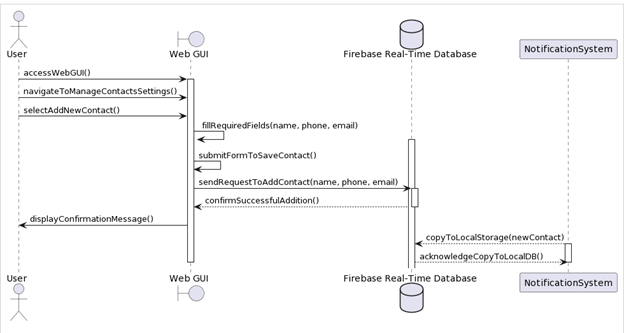
\includegraphics[width=\imagewidth]{../assets/sequence/AddingNewContactInformationSequenceDiagram.png}
    \caption{The sequence diagram for the adding new contact information use case.}
    \label{fig:add-contact}
\end{figure}

\section{Schematics}

\begin{figure}[H]
    \centering
    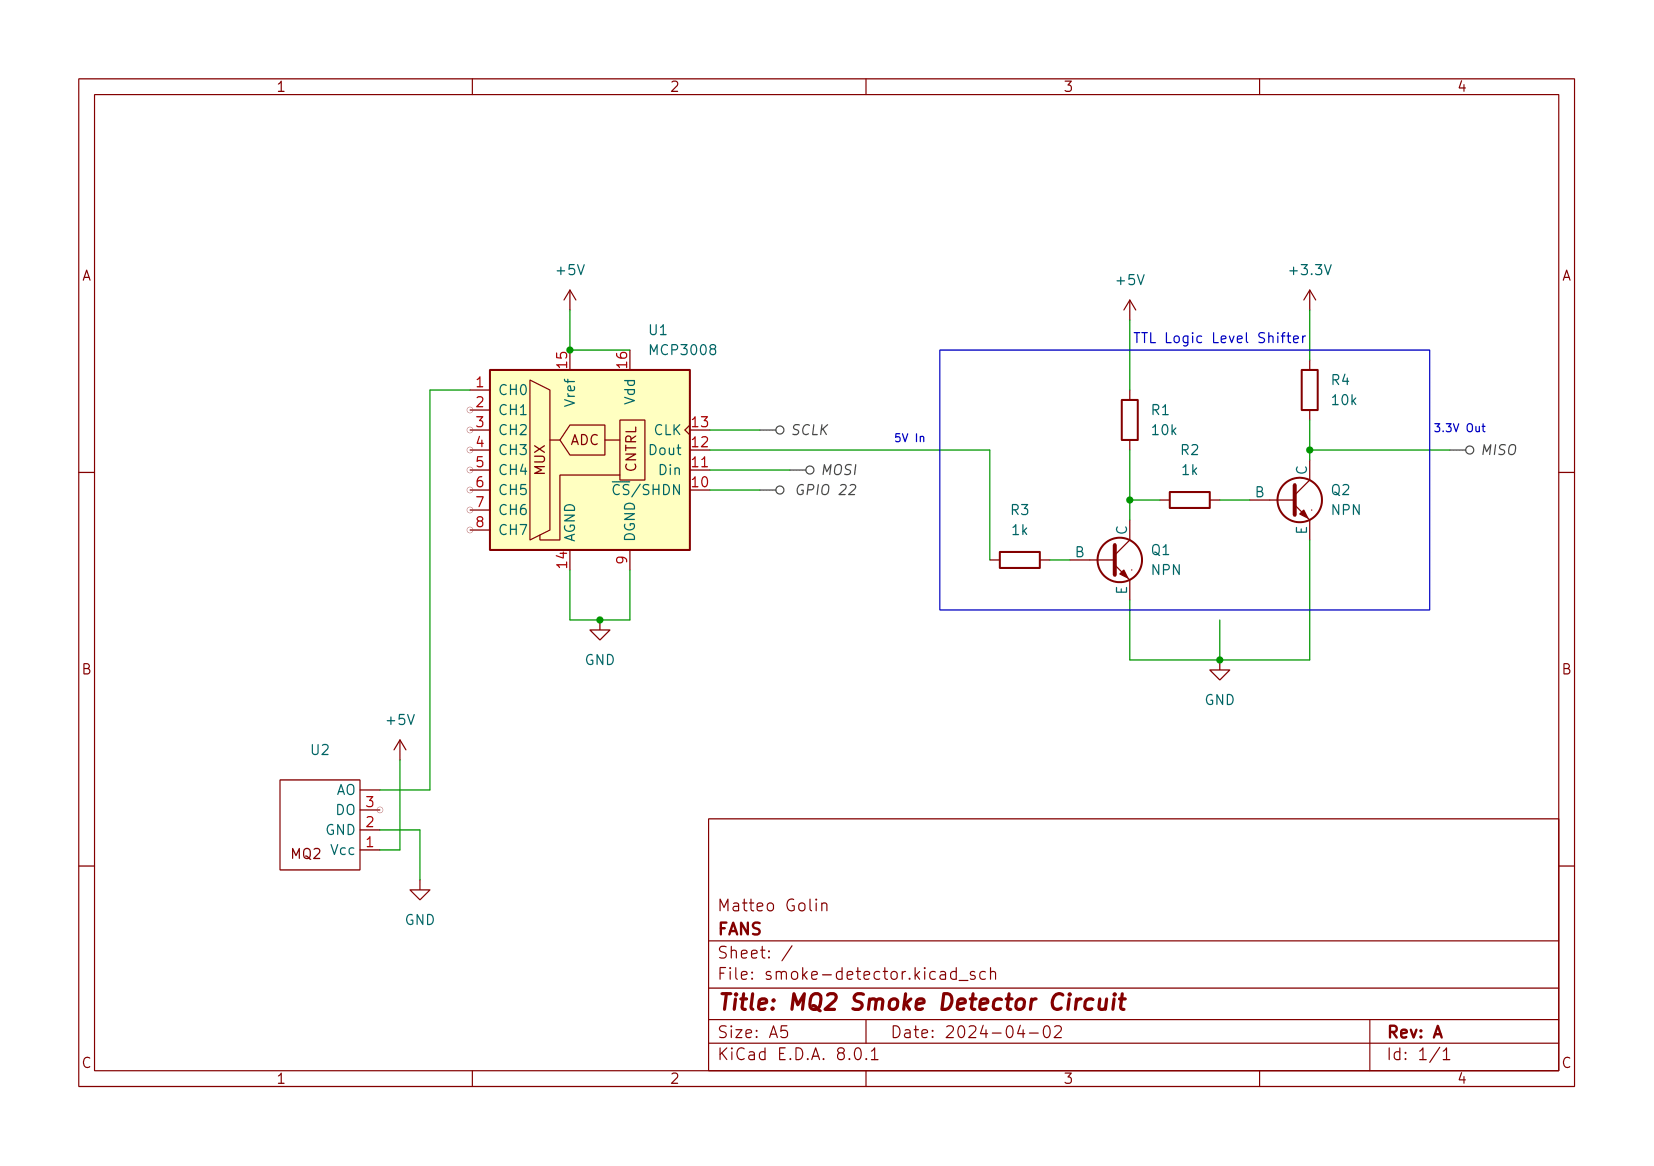
\includegraphics[width=5in]{../assets/schematics/MQ2-Schematic-Final.png}
    \caption{The smoke detection system's electrical connections.}
\end{figure}

\begin{figure}[H]
    \centering
    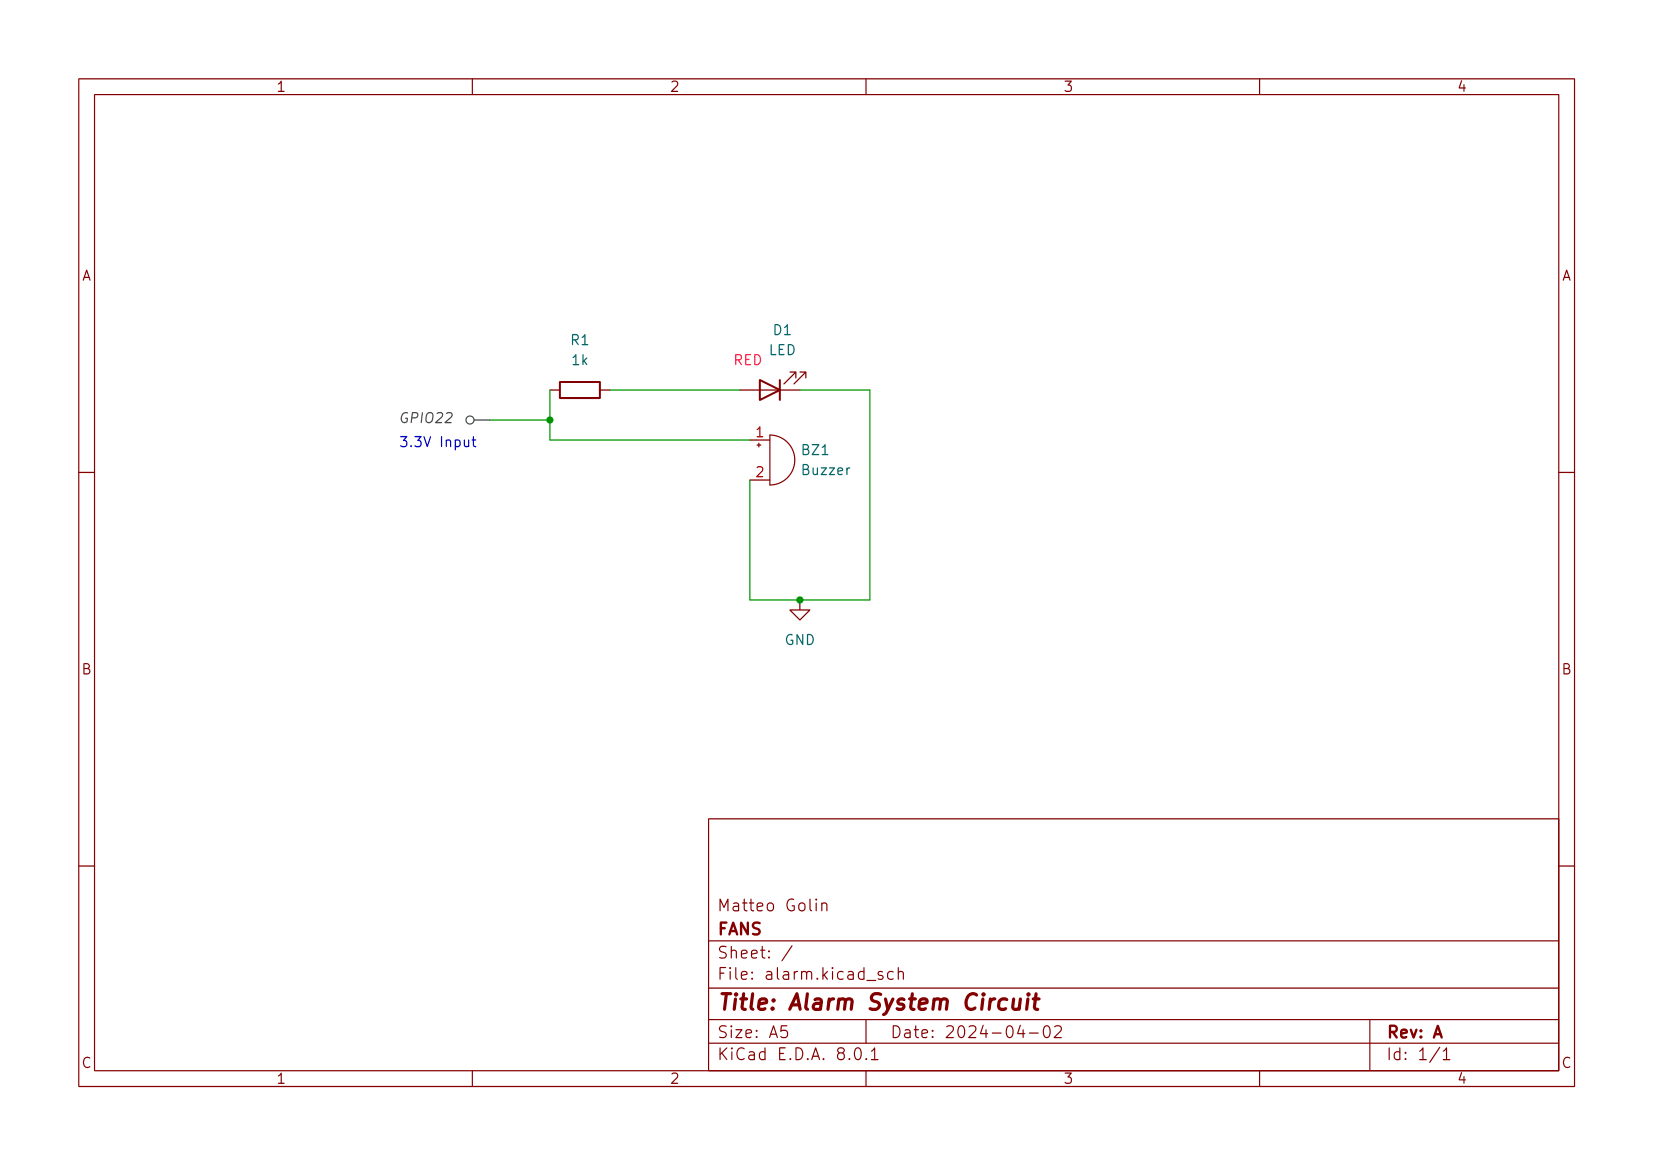
\includegraphics[width=5in]{../assets/schematics/Alarm-Schematic.png}
    \caption{The alarm system's electrical connections.}
\end{figure}

\begin{figure}[H]
    \centering
    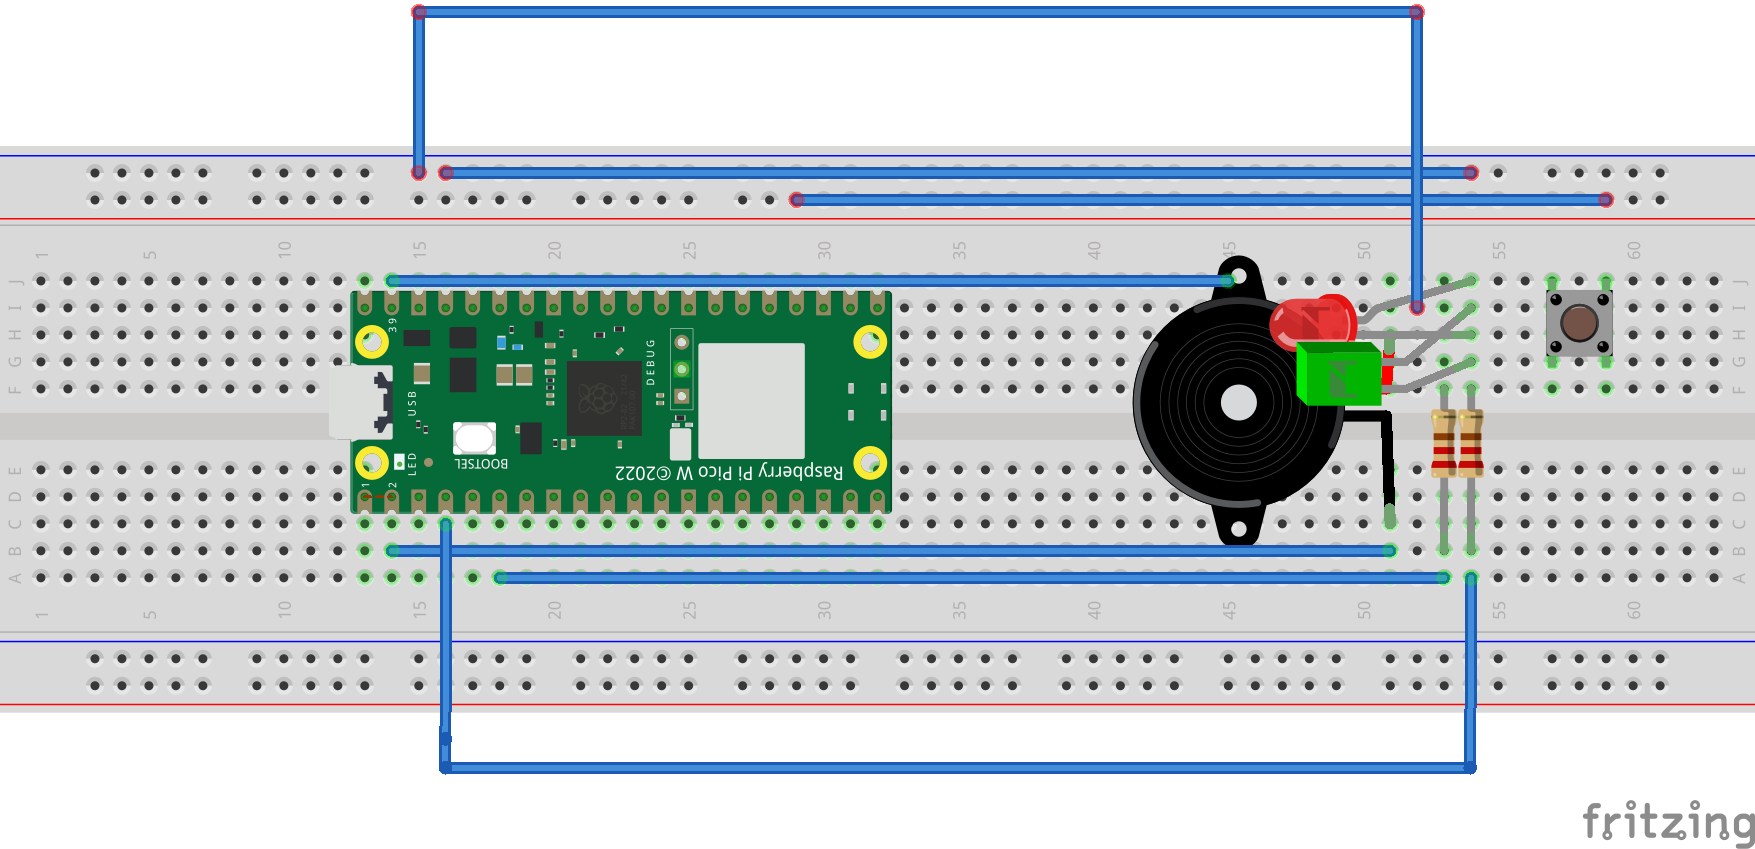
\includegraphics[width=5in]{../assets/schematics/fritzingpico.png}
    \caption{The haptic alarm system's wiring diagram on a breadboard.}
\end{figure}

\section{State Machine Diagrams}

\subsection{Alarm System}

\begin{figure}[H]
    \centering
    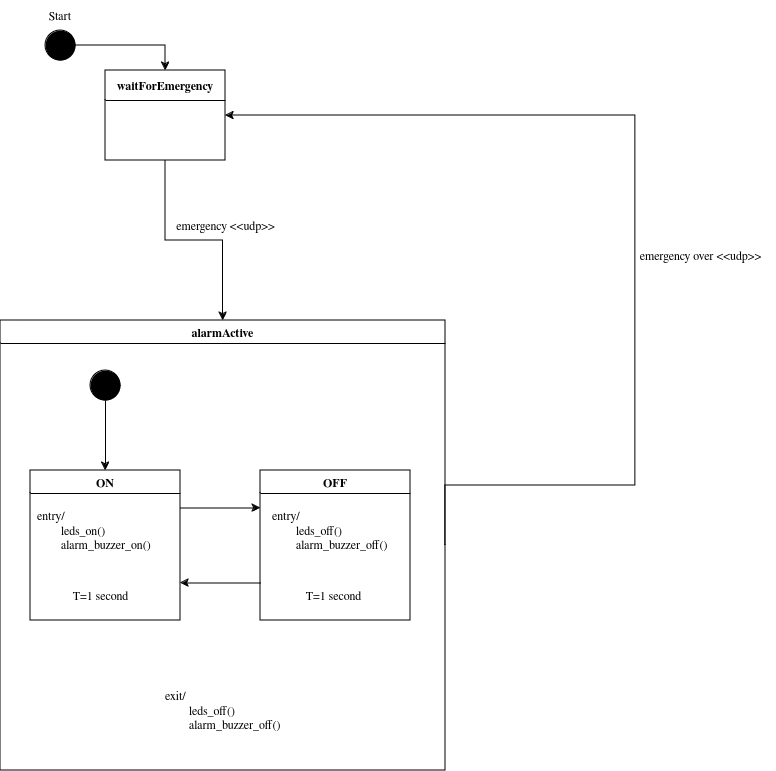
\includegraphics[width=5in]{../assets/state-machine/AlarmSystemStateMachine.png}
    \caption{The alarm system's software state machine.}
\end{figure}

\subsection{Smoke Detection System}

\begin{figure}[H]
    \centering
    
\includegraphics[width=4in]{../assets/state-machine/DataCollectionStateMachine.png}
    \caption{The smoke detection system's software state machine for data collection.}
\end{figure}

\begin{figure}[H]
    \centering
    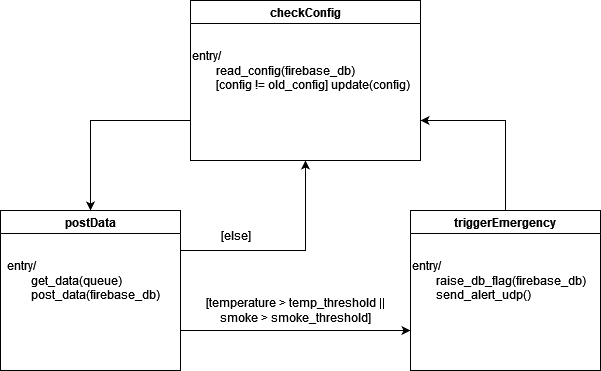
\includegraphics[width=4in]{../assets/state-machine/DataCollectionLogicLoop.png}
    \caption{The smoke detection system's software state machine for performing its primary logic.}
\end{figure}

\subsection{Notification System}

\begin{figure}[H]
    \centering
    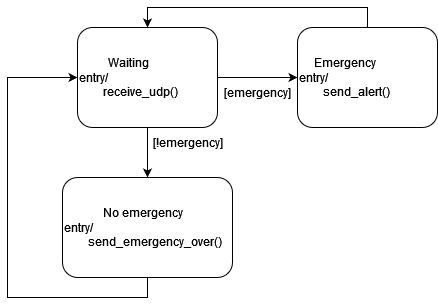
\includegraphics[width=4in]{../assets/state-machine/NotificationSystemStateMachine.png}
    \caption{The primary logic of the notification system as a state machine.}
\end{figure}

\subsection{Haptic Alarm}

\begin{figure}[H]
    \centering
    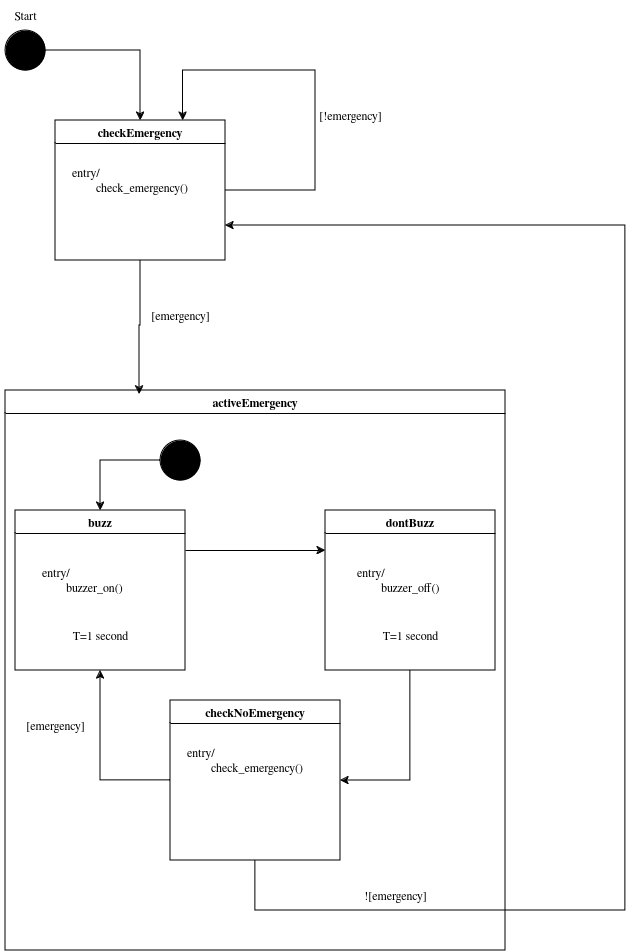
\includegraphics[width=4in]{../assets/state-machine/HapticAlarmStateMachine.png}
    \caption{The primary logic of the haptic alarm as a state machine.}
\end{figure}


\end{document}
